%!TeX root=./tese.tex
% Closed-loop chapter. Every number is ledgered in progress/results-ledger.md:
% "4.4 fleet matrix", "4.4 rider (d) detection", "4.4 LLM forecast closed
% loop under realistic leads", "4.4 weekly aggregate", "Principled LLM
% capacity mapping", "Encoder model-side cold start (Phase D)".
% Artifacts: simulation/results/results_44.jsonl, riders44/, aggregate44/.
\chapter{Closing the Loop: Forecast-Driven Per-Pool Provisioning}
\label{cap:closedloop}
\chaptermark{Forecast-Driven Provisioning}

This chapter delivers the thesis's contribution proper: per-pool worker
schedules driven by the zero-shot forecasts of
Chapter~\ref{cap:predictors}, executed on the platform of
Chapter~\ref{cap:twopool}, and scored against the baselines of
Chapter~\ref{cap:baselines} under the same SLA, windows, actuation, and
cold-start leads. The design questions are answered by ablation:
headroom quantile (p50 versus p90), forecasting model (three TSFMs),
capacity rating $\rho$, and per-pool cold-start lead $L$. The
chapter closes with the week-scale aggregate that prices the policy
against the deployable static fleet.

\section{From forecast to worker schedule}
\label{sec:cl-controller}

The controller is deliberately minimal, so any advantage traces to
the information source, not control sophistication. For the \emph{encoder pool}, the archived stitched
forecast path of the image-rate signal (15-second bins, rolling
origin) is read at
quantile $q$, converted to a worker count
$C(t) = \lceil \hat{y}_q(t) / \rho \rceil$ at per-worker capacity rating
$\rho$ \si{img/s}, and actuated with cold-start lead $L$ (the schedule
is \emph{issued} $L$ early, precisely what a forecast permits) and
3-minute scale-down hysteresis. These are the same law, lead, and hysteresis
as the reactive strawman of
Section~\ref{sec:base-reactive-enc}, which reads the trailing observed
\emph{point} rate (quantile ignored) rather than the p90 forecast band;
the raw head-to-head therefore bundles anticipation with headroom, and the two
dials are separated by the p50-forecast, lead-invariance, and
reactive-with-headroom ablations below. For the \emph{language
pool}, the forecast path replaces the planner's built-in predictor
inside Dynamo's SLA-planner loop (a \texttt{forecast\_file}
predictor registered in the planner's registry), so
predictive and reactive language-pool policies share the production
actuation path end to end; replica lead is enforced by the simulator's
native worker-startup delay.

\paragraph{Temporal split.} The trace's
first 1.4 days are consumed as forecast \emph{context}, the
zero-shot models' rolling history before their first usable
15-second forecast, and are never graded; the remaining 5.60 days
form the evaluation span, on which every closed-loop verdict in this
chapter is scored (episodes burst1/3/4/5 and the calm day; the two
pre-coverage episodes are graded only by forecast-free policies,
Chapter~\ref{cap:baselines}). No information flows backward across the
split or within it: every forecast value is issued at or before the
bin it predicts --- issue time $=$ target $-\,(h{-}1){\cdot}15$\,s, so
the $h{=}1$ nowcast carries zero usable lead and longer horizons
strictly precede (rolling origin, Chapter~\ref{cap:predictors}) --- and
no policy constant is \emph{tuned} on the evaluation span. Each
is either derived from capacity measurement (the encoder cost model,
the belief-to-knee conversion) or swept with all values reported
(headroom quantile, capacity rating, cold-start leads); the headline
rating $\rho{=}15$ is then chosen \emph{ex post} as the conservative
operating point (Section~\ref{sec:cl-aggregate} shows $\rho{=}20$ also
clean, more cheaply), with the whole frontier reported rather than a
value selected to flatter the result. A deployed
system would enter the week with prior history as context; the warm-up
hole is the price of zero-shot honesty, not a property of the method.

\section{Encoder pool: the lead-time result}
\label{sec:cl-matrix}

The p90-forecast policy at $\rho{=}15$ is graded on a per-window
factorial --- 5 in-span windows $\times$ 3 TSFMs $\times$ 4 realizable
issued leads $\{15,30,45,165\}$\,s, each a two-pool replay rebuilt under
\emph{issue-time} actuation (honouring the archive's tiled issue times) ---
and \textbf{meets the SLA in all 60 of its cells: every window, every
model, every lead}, under \emph{both} a warm-pool and a strict re-warm
readiness model (the four burst windows pinned at the
\SI{588}{\milli\second} service floor; the calm day 548--\SI{734}{\milli\second}).
The broader exploratory grid that located this operating point (adding
p50, the reactive baseline, four capacity ratings, and a non-realizable
\SI{300}{\second} target-time lead; 560 target-time cells) is superseded
for the forecast headline by this issue-time rebuild: the H=12 15-second
archive supplies at most $(12{-}1)\times15 = \SI{165}{\second}$ of
forecast-issued lead, and the \SI{300}{\second} cell reached the same
floor only by target-time indexing --- an upper bound, not an issued
lead. By contrast, the identically
informed reactive controller loses burst3 at every lead and
burst4/5 beyond 45 seconds (Table~\ref{tab:base-react-enc}). On the
burst windows the p90 schedule's p99 encoder delay is pinned at
\SI{588}{\milli\second}, exactly the platform's zero-queueing
service floor: a full-batch forward ($f(64) =$
\SI{316.4}{\milli\second}) plus the p99 handoff transfer
(\SI{272}{\milli\second}). Anticipated capacity removes
queueing entirely, and what remains is physics.

The ablations locate why, and what each dial buys:

\begin{description}
\item[Quantile is the decisive dial.] The p50 policy is not viable: at
$\rho{=}15$ it clears only 23--24 of its 60 issue-time cells (24 under
the warm-pool readiness model, 23 under strict re-warm) and fails even
the calm day (p99 \SI{1073}{\milli\second} at every lead and model: the
median forecast sizes to the mean, allocates one worker, and reproduces
on the vision pool the reactive planner's mean-sizing defect). The calibrated p90 band edge
(Chapter~\ref{cap:predictors}: empirical coverage 0.88--0.90 at this
cadence) is what converts a point forecast into provisionable headroom.
\item[Lead-invariance is the signature of anticipation.] Actuated on
true forecast issue time (each 180-second tile's 12-step forecast ordered
at its origin, honouring issue $\le$ decision), the p90 policy holds its
per-window p99 unchanged across leads from $L{=}15$ to \SI{165}{\second}
--- the archive's maximum issued lead --- at the \SI{588}{\milli\second}
service floor on every burst window and feasible (below
\SI{734}{\milli\second}) on the calm day, while the
reactive twin degrades monotonically with
lead toward its never-scaled limit (burst3: 9{,}481 to
54{,}170\,\si{\milli\second}). A policy that must \emph{observe} an
onset pays for lead; a policy that provisions from an already-issued
forecast band does not, up to the lead the archive supplies. (This is a
\emph{feasibility} invariance: the \SI{588}{\milli\second} floor holds
under both a warm-pool and a strict re-warm readiness model; the
provisioned \emph{cost} is flat under the former and mildly
lead-dependent, 0.59--0.62$\times$, under the latter ---
Section~\ref{sec:cl-aggregate}.)
\item[Model choice is second-order.] All three foundation models pass
all 60 p90/$\rho{15}$ cells, consistent with the small cross-model
spreads of Chapter~\ref{cap:predictors}. The same holds for
the predictor a production planner ships: swapping Dynamo's own load
predictor among ARIMA, Kalman, and Prophet leaves the SLA verdict
unchanged on both a decode-bound day and a slow-onset burst (identical
served-latency percentiles on the former, within \SI{1}{\milli\second}
of mean TTFT on the latter, all failing together), because the
integer-replica conversion quantizes the differing forecasts onto the
same worker schedule. Predictor choice is second-order \emph{within} the foundation-model and
shipped-predictor families; the signal, the conversion, and --- across the
wider forecaster class --- the calibrated band \emph{shape} are not
(Table~\ref{tab:cl-ewma}).
\item[Capacity rating trades cost against fragility.] At $\rho \in
\{10,15,20\}$ the p90 policy is \emph{60/60} on the issue-time factorial
under both readiness models, though margin tightens with $\rho$
(per-window p99 rises from the \SI{588}{\milli\second} floor to
\SI{746}{}/\SI{860}{\milli\second} warm/strict at $\rho{=}20$); only
$\rho{=}25$ drops cells --- 9 of 60, all on burst5, the binding static
window, via backlog it never drains. The reactive policy, by contrast,
is insensitive to $\rho$ (13--14 of 20 cells at every rating): no
capacity rating repairs late information.
\end{description}

\paragraph{Mechanism: graduated headroom, not clean detection.}
Reading the archived forecast paths as a burst detector, restricted to
each declared episode and scored at true forecast issue time, the p90
band crosses \emph{ahead} of the observed rate on burst4 (by
\SI{225}{\second} at the \SI{224}{img/s} one-minute-p99 threshold, a
\SI{345}{\second} usable issue-lead, and still ahead at the tighter
\SI{286}{img/s} 15-second-cadence threshold) and --- at the one-minute
threshold only --- on burst5 (by \SI{105}{\second}; under the tighter
15-second threshold burst5 lags), but \emph{lags} on the fastest onset
(burst3, issued at $h{=}1$, no usable lead) and on burst1's first
in-episode crossing. The
closed-loop pass on burst3 therefore does not rest on clean pre-signal
detection --- the forecast lags the onset (issued at $h{=}1$). It rests on
the p90 band's \emph{graduated headroom}: the calibrated band already sits
elevated during the ambient activity \emph{before} the spike (the
permissive, over-provisioning behaviour the $\rho$-frontier already
prices), lifting provisioned capacity to ${\approx}21$ workers, so capacity
is standing when the one-minute spike lands --- the near-term nowcast adding
at most the cold-start lead of placement, not the several minutes an onset
this fast would need to be caught by detection. This is standing headroom
read as a provisioning signal, not onset anticipation. The point and p50 paths, sizing to the mean, detect the same
onsets 55 minutes to 4 hours late, or never; and the p90 band shows zero
false alarms across the calm day for every model.

A binary reading of the detector must be qualified, though. Counting
threshold crossings over the \emph{whole} 5.60-day span (outside the
true episodes), the p90 path crosses on 70--102 bins per day where the
observed rate does not, while point and p50 cross essentially never
($\leq$1 per day). Read as an alarm, p90 is trigger-happy; but it is
used as the \emph{provisioning quantile}, not an alarm, and a band that
sits above the burst threshold during moderate activity is the
calibrated headroom (coverage 0.88--0.90, Chapter~\ref{cap:predictors})
doing its job: over-provisioning slightly, exactly the cost the
$\rho$-frontier already prices (the per-episode-clean band
$\rho\in\{10,15,20\}$ costs 0.48--0.89$\times$ static). The
distinction is the point: p90 is a good provisioning signal precisely
\emph{because} it is a permissive detector --- not a generic safety
margin but, at provisioning cadence, a calibrated early-warning channel
whose cost is accounted for. Point and p50 are the opposite, clean detectors
that fail as provisioning signals, sizing to the mean and missing the
onset.

\paragraph{Anticipation versus headroom, separated directly.} The raw
forecast-versus-reactive contrast changes two dials at once --- the
forecast both looks ahead and reads a p90 band, while the reactive
strawman reads a trailing \emph{point} rate. To isolate them we run the
reactive controller with the tail-aware headroom it was denied: the
trailing-window p90 of the observed image rate (windows of 2--8\,min) at
the same $\rho{=}15$ and lead, but still no forecast. On the slow onset
(burst1) and at week scale this reactive-with-headroom controller passes,
as the point reactive already does; but on the one-minute onset (burst3)
it fails at every lead and window (p99 $1{,}973$--$11{,}568$\,\si{\milli\second}
against the forecast's \SI{588}{\milli\second}), even though the headroom
cuts its p99 up to $8\times$ below the point reactive. Tail-aware headroom
is therefore necessary but not sufficient on a fast onset: calibrated to
past load, it cannot stand up the replicas a sub-minute spike demands,
which only a forward forecast band places ahead of the onset. The
p90-forecast's fast-onset win is thus the forward band's better-placed
standing headroom, not onset foresight --- genuine anticipatory lead is
measured only on the gradual onset (burst4, ${+}\SI{345}{\second}$); the
trailing-window headroom, at equal $\rho$, cannot match that placement on a
sub-minute onset.

\paragraph{A cheap forward forecaster does not get the result for free.}
The accuracy benchmark's near-parity (Chapter~\ref{cap:predictors}) raises the
question of whether the foundation model is load-bearing at all, or whether a
classical \emph{forward} forecaster at a calibrated quantile would reproduce
the headline. It does not (Table~\ref{tab:cl-ewma}). Driving the identical
encoder loop with a forward EWMA point path --- its p90 empirically calibrated
on the 1.4-day forecast-context window to the same 0.88--0.90 coverage as the
foundation-model band, by three standard schemes (additive and multiplicative
split-conformal, and a width-scaled native band) --- exposes a
coverage-versus-cost bind. The two cheap calibrations clear the
\emph{burst-masked} week aggregate (0.70$\times$ and 0.56$\times$, both at
aggregate p99 \SI{589}{\milli\second}) but \emph{fail} the fast onset (burst3
p99 1{,}285 and 2{,}084\,\si{\milli\second}) and the high-volume onset
(burst5, backlog-divergent) under per-episode grading --- the same
dashboard-masking the reactive baseline shows (Section~\ref{sec:cl-aggregate}),
now on a forward forecaster. The one calibration that clears every episode
(multiplicative, burst3 \SI{747}{\milli\second}) over-provisions moderate
activity and costs 1.09$\times$ static, and only at $\rho{\geq}20$ does it
come under the static fleet at all ($\rho$-frontier 1.32/1.09/0.94/0.83$\times$
at $\rho\in\{10,15,20,25\}$) --- and $\rho{=}25$ is where even the foundation
policy loses burst5. Only the zero-shot foundation-model band clears every
episode \emph{and} beats static (0.62$\times$). The refinement of ``model
choice is second-order'' is thus precise: forecast \emph{accuracy} is
second-order (ARIMA ties Chronos, Chapter~\ref{cap:predictors}), but the
calibrated p90 band \emph{shape} is not --- a state-adaptive band that lifts
at onsets without inflating in calm is what simultaneously holds the tail and
stays cheap, and it is what the foundation models supply zero-shot while
standard forward-EWMA calibrations do not. The Chronos control reproduces the
committed figures to within run noise ($<1\%$) throughout (burst3
\SI{588}{\milli\second}; week 0.62$\times$; $\rho$-frontier
0.89/0.62/0.48/0.40$\times$; the p50 arm
fails at \SI{2735}{\milli\second}/0.25$\times$; archive
\texttt{verification/results/ewma\_sweep.json}).

\begin{table}[htbp]
\centering
\caption{Forward-EWMA calibrated-p90 versus the foundation-model policy
through the \emph{identical} encoder loop ($\rho{=}15$, issue-time actuation,
warm-pool; each EWMA p90 calibrated on the 1.4-day context to 0.88--0.90
coverage). Per-window encoder-delay p99 is lead-invariant over
$L\in\{15,\ldots,165\}$\,s; ``agg'' is the week-scale cost versus the
deployable static $C{=}8$ fleet. \emph{Every} policy clears the aggregate p99
at the \SI{589}{\milli\second} service floor --- the burst-masking of
Section~\ref{sec:cl-aggregate} --- so the operative verdict is per-episode.}
\label{tab:cl-ewma}
\small
\begin{tabular}{@{}lrrrrrrl@{}}
\toprule
Forecaster (p90) & burst1 & burst3 & burst4 & burst5 & steady & agg &
per-episode \\
 & \multicolumn{5}{c}{encoder-delay p99 (\si{\milli\second})} &
$\times$static & verdict \\
\midrule
Foundation (Chronos)  & 589 & 589             & 589 & 589            & 681 & 0.62 & \textbf{pass all} \\
EWMA, add-conformal   & 658 & \textbf{1{,}285}& 589 & div$^\dagger$  & 418 & 0.70 & fail b3,\,b5 \\
EWMA, mult-conformal  & 589 & 747             & 589 & 589            & 418 & 1.09 & pass all \\
EWMA, width-scaled    & 611 & \textbf{2{,}084}& 589 & div$^\dagger$  & 736 & 0.56 & fail b3,\,b5 \\
\bottomrule
\end{tabular}

\vspace{2pt}
{\footnotesize $^\dagger$ backlog-divergent (the queue never drains): a hard
SLA failure, distinct from a finite tail over the bound.}
\end{table}

\section{Language pool: the conversion result}
\label{sec:cl-llm}

On the language pool, with the forecast feeding Dynamo's planner and
replicas subject to realistic startup leads of 60--300 seconds, the
policy passes the burst window at every lead (TTFT p99 736--757\,\si{\milli\second}, ITL p99
${\approx}$\SI{6.5}{\milli\second}, versus
\SI{751}{\milli\second} with instant workers): lead-invariant on this
pool as well, though for a different reason. (The language forecast hook
consumes a fixed per-tick cursor --- the current forecast tile's target
bin, not a re-issued origin --- so this pool tests the \emph{conversion}
under a held forecast signal rather than language-side anticipation; the
anticipation result is the encoder pool's, and this pool's insensitivity
to replica lead is a property of the tail-aware conversion, not of a
second scale-ahead controller. Concretely the hook, starting one minute
before $T_0$, reads a \emph{single} 15-second forecast bin per planner
tick --- the bin at tick index $4t$, its value pre-scaled to the tick's
60-second rate --- and steps four bins (one minute) per tick: it
\emph{samples} one bin per control minute rather than aggregating the
minute's four bins. This is adequate for the conversion comparison it
supports but is not a timing or anticipation instrument, so the
language-pool result is best read as a synthetic sampled-signal
experiment.) The pass has a second
necessary ingredient: a \emph{tail-aware capacity conversion}. Run with
the planner's native conversion (replicas $=$ mean demand over mean
per-replica throughput), the \emph{same forecast} fails much like the
reactive baseline, marginally worse
(Table~\ref{tab:cl-triad}): signal quality
cannot compensate for a mean-to-tail conversion error.

\begin{table}[htbp]
\centering
\caption{The two ingredients, separated (burst1, replica lead
\SI{60}{\second}): the forecast alone does not pass; the forecast plus a
tail-aware capacity conversion does.}
\label{tab:cl-triad}
\small
\begin{tabular}{@{}lrrl@{}}
\toprule
Policy & TTFT p99 (ms) & ITL p99 (ms) & Verdict \\
\midrule
Reactive planner (best ladder point) & 1{,}615.5 & 125.1 & FAIL \\
Forecast, mean-based conversion & 1{,}716.6 & 126.8 & FAIL \\
Forecast, tail-aware conversion & 736.3 & 6.3 & PASS \\
\bottomrule
\end{tabular}
\end{table}

The tail-aware conversion is derived, not tuned. The planner sizes
replicas as $\lceil \hat{d} / \hat{r} \rceil$ where $\hat{r}$ is its
belief about per-replica throughput (measured in-loop: median
\SI{10.07}{req/s} per TP2 replica); the SLA-relevant capacity is instead
the measured \emph{tail knee} $r_{\text{tail}}$: the largest offered
rate a replica sustains under the tail SLA
(\SI{1.62}{req/s} on burst1's mix; bracketed in $[1.26, 1.44]$ on
burst4, the binding mix). Scaling the forecast by
$\hat{r}/r_{\text{tail}}$ makes the mean-based planner land on
tail-adequate replica counts, and validation flips exactly at the
formula's boundary on both windows tested (burst1: scale 4.64 fails,
6.22 passes at $-16\%$ GPU-hours versus the conservative setting;
burst4: 6.22 fails, 7.0 passes). A ${\approx}14\%$ margin above the
binding knee is retained as policy, since $r_{\text{tail}}$ is
mix-dependent and planner-in-loop replays show ${\approx}4\%$ p99 run
noise. On burst windows the resulting language fleet costs about what
the static optimum does, and correctly so, since the static optimum is
burst-sized. The language-side saving is cross-window (TP1$\times$2 on
calm traffic, half the burst fleet's GPUs), while the decisive per-pool
savings are on the encoder side, priced next.

\paragraph{The quantile dial, on the language pool too.} On burst1's
slow onset the p50 forecast sufficed; on the fastest onset it does not.
Replaying burst3 end-to-end (60-second replica lead, tail-aware
conversion throughout) yields the language-pool mirror of the encoder
matrix's quantile result: reactive fails at TTFT p99
3{,}495\,\si{\milli\second}; the p50 forecast fails at
2{,}164\,\si{\milli\second} (better-informed but still
under-provisioned: at a held forecast cursor the p50 band sizes to the
mean, the same mean-to-tail conversion defect the encoder matrix shows,
not a timing lag on this pool);
and the p90 forecast passes at \SI{651}{\milli\second}. Headroom
quantile, not signal access, separates pass from fail on fast onsets on
\emph{both} pools --- on the language pool this is the conversion dial
under a held forecast cursor, not a second anticipation test. (This
burst3 configuration is also the policy pair
carried to the live-stack validation of Chapter~\ref{cap:validation}.)
The verdict is not particular to burst3: replaying every burst episode
end-to-end, the p90 forecast passes each one at the service floor
(TTFT p99 651--706\,\si{\milli\second} across onsets of 1--220 minutes)
while the reactive planner fails all four
(1{,}615--3{,}495\,\si{\milli\second}).

\paragraph{The language pool at week scale.} In a continuous replay of
the full 5.60-day evaluation span through the planner (the composed
trace under the winning encoder schedule, 60-second replica lead), the
p90-forecast policy \textbf{passes the week} at TTFT p99
\SI{651}{\milli\second}
(ITL p99 \SI{6.4}{\milli\second}) for 518.6 H100 GPU-hours, slightly
below the burst-sized static TP2$\times$2 fleet's 537.4 for the same
span (0.96$\times$; replica scaling cannot morph TP2 into TP1, so the
language pool's dynamic savings are structurally small). The week
verdict is
forecast-model-independent: replacing Chronos with Toto or TimesFM holds
the tail at the identical \SI{651}{\milli\second} (both pass), shifting
only the provisioning cost (625 and 641 versus 518.6 GPU-hours ---
1.16$\times$ and 1.19$\times$ the burst-static fleet, so the language
pool's near-break-even cost is Chronos-specific; the pass/fail
\emph{verdict} is model-independent among the foundation models, the cost is not). The forecast
model sets how much headroom is bought, not whether the SLA is met. The reactive planner \textbf{fails the
week outright} (TTFT p99 1{,}197\,\si{\milli\second}) while spending
281.8 GPU-hours: half the budget, and the wrong tail. At week scale
as at window scale, spend is not the defect.

The quantile matters less here than on the encoder pool, and the
contrast is diagnostic. The p50 forecast also \textbf{passes the week}
on the language pool (TTFT p99 \SI{828}{\milli\second}, for 319.9
GPU-hours: 38\% cheaper than p90, with correspondingly less tail
headroom), whereas on the encoder pool p50 fails every one of its 48
week-scale cells. The mechanism is the burstiness gap: the tail-aware
conversion is applied to both forecasts, but image demand is bursty
enough that a median forecast's mean-sizing floods the encoder FIFO,
while the smoother context-token demand is served adequately even at
p50 once the conversion supplies enough replicas. What is universal
across pools is the \emph{conversion}: mean-based reactive control
fails both, tail-aware forecast control passes both. What is
pool-specific is how much the \emph{quantile} adds, and it adds most
where the signal is burstiest.

\begin{figure}[htbp]
\centering
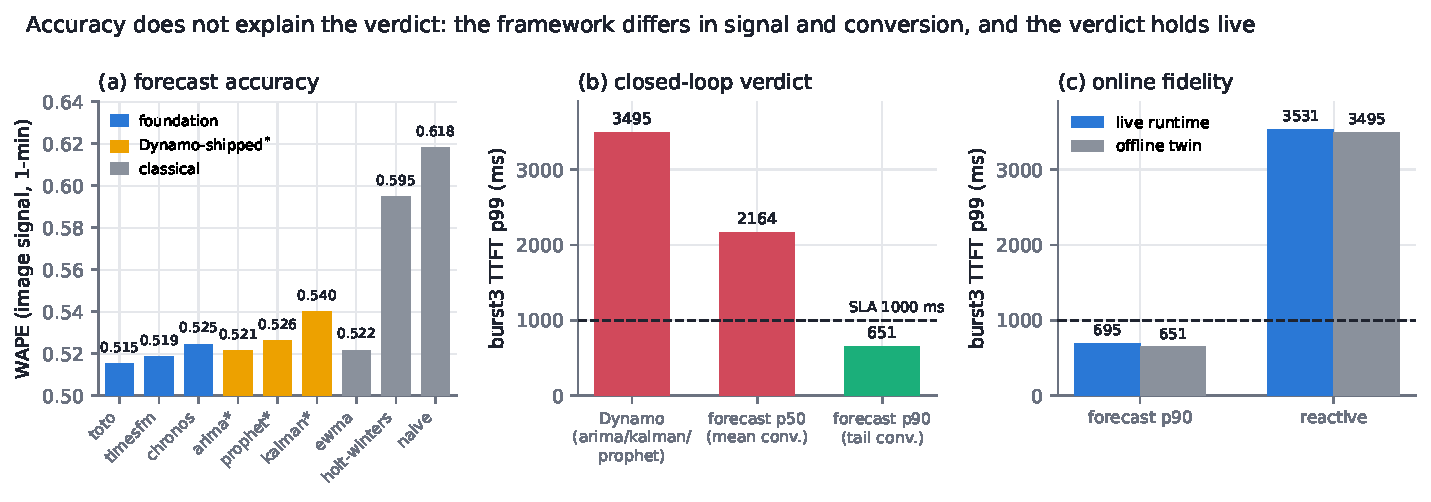
\includegraphics[width=\linewidth]{figuras/pred/pred_framework_diff}
\caption{Why the framework differs, in three measurements.
\textbf{(a)} On the image signal at provisioning cadence the predictors
are near-parity: the foundation models (blue) and Dynamo's shipped
predictors (yellow: ARIMA, Prophet, Kalman) cluster within
$0.02$ WAPE, and ARIMA ties Chronos. Accuracy alone does not separate
them. \textbf{(b)} Yet on the burst3 closed loop the verdict is
categorical: every mean-conversion policy fails the SLA, Dynamo's
shipped predictors (\SI{3{,}495}{\milli\second}, forecaster-invariant)
and the forecast at the median quantile
(\SI{2{,}164}{\milli\second}) alike, while only the p90 forecast
\emph{with a tail-aware conversion} passes (\SI{651}{\milli\second}).
The differentiator is the signal and the conversion, not forecast
accuracy. \textbf{(c)} And the verdict holds on the live Dynamo runtime:
both policies' online TTFT tails track their offline twins
directionally, within 1.1--6.8\% (Chapter~\ref{cap:validation}; a single
live run per policy, not a repeated-trial noise band).}
\label{fig:cl-framework-diff}
\end{figure}

\section{The week-scale aggregate}
\label{sec:cl-aggregate}

The final experiment prices the encoder-pool policy over the full
forecast-covered span (5.60 continuous days, 749{,}601 requests,
11.4M images, containing four of the six burst episodes and the calm
day) against the deployable static fleet of
Chapter~\ref{cap:baselines} (Table~\ref{tab:cl-aggregate}).

\begin{table}[htbp]
\centering
\caption{Week-scale aggregate (5.60-day covered span, 749{,}601
requests): encoder-delay p99, provisioned worker-time, and per-episode
compliance. ``Episodes'' grades each in-span burst episode separately
(the aggregate p99 alone can mask sub-1\% episodes). Forecast policies
use Chronos-2 at $\rho{=}15$; $L$ is the cold-start lead. Forecast
worker-time is actuated on forecast \emph{issue} time (each 180-second
tile's 12-step forecast is ordered at its origin, honouring
issue~$\le$~decision) and, under the warm-pool readiness model, is
lead-invariant across the archive's realizable 15--\SI{165}{\second}
issued-lead range (2.41M at both ends; 0.59--0.62$\times$ under strict
re-warm, see text);
indexing by \emph{target} time instead --- assuming capacity placed
exactly at each bin rather than ordered at forecast-issue time --- is an
optimistic bound, cheaper at longer, less-realizable leads (2.38M at
$L{=}30$ down to 2.12M at the non-realizable $L{=}300$). The three
rows reading \SI{588}{\milli\second} are distinct runs (their
worker-time and worst-case delay differ) that coincide at the
zero-queueing service floor: a full-batch forward
($f(64)=\SI{316.4}{\milli\second}$) plus the p99 handoff
(\SI{272}{\milli\second}), which every adequately provisioned policy
reaches because all share the same encoder. Rows above it
(\SI{644}{\milli\second} and up) carry queueing on top of that floor.}
\label{tab:cl-aggregate}
\small
\begin{tabular}{@{}lrrrl@{}}
\toprule
Policy & p99 (ms) & Mworker-s & vs.\ static & Episodes \\
\midrule
Static $C{=}8$ (deployable) & 644 & 3.87 & 1.00$\times$ & pass \\
Static $C{=}2$ (calm-day optimum) & \textbf{2{,}953} & 0.97 &
0.25$\times$ & fail \\
Forecast p90, $L{=}30$\,s (issue-time) & 588 & 2.41 & 0.62$\times$ & pass \\
Forecast p90, $L{=}165$\,s (issue-time, max) & 588 & 2.41 & 0.62$\times$ & pass \\
Forecast p50, $L{=}30$\,s & \textbf{2{,}735} & 0.98 & 0.25$\times$ &
fail \\
Reactive, $L{=}30$\,s & 588 & 2.61 & 0.67$\times$ & \textbf{fails
burst3} \\
Reactive, $L{=}300$\,s & 905 & 1.67 & 0.43$\times$ & \textbf{fails
burst3} \\
\bottomrule
\end{tabular}
\end{table}

The headline: \textbf{the p90-forecast schedule meets the tail SLA over
the aggregate \emph{and} inside every in-span episode at 0.62
times the deployable static encoder fleet's provisioned worker-time}
(2.41M worker-seconds versus 3.87M, at p99 \SI{588}{\milli\second}
versus the static fleet's 644). Actuated on forecast issue time
(each 180-second tile's forecast ordered at its origin,
issue~$\le$~decision), the cost is essentially lead-invariant across the
archive's realizable 15--\SI{165}{\second} issued-lead range (2.41M at
both ends): it is the tiled forecast's availability, not the nominal
lead, that bounds how early capacity can be ordered. Indexing by target
time instead is an optimistic bound that grows cheaper at longer,
less-realizable leads (2.38M at $L{=}30$ to 2.12M at the non-realizable
$L{=}300$), and no issue-time schedule realizes it. This flatness
assumes a \emph{warm-pool} readiness model: a scaled-down replica can
return without re-paying cold start, which matches the converter's LIFO
slot reactivation and a deployed rolling-origin controller that
re-forecasts every level within its horizon. Under a strict re-warm
model instead --- a retired replica re-orders and re-pays lead --- the
cost is mildly lead-dependent (0.62$\times$ at $L{=}15$ falling to
0.59$\times$ at $L{=}165$), still passing at the \SI{588}{\milli\second}
floor at every lead; \textbf{0.62$\times$} is therefore the conservative
figure across both readiness models, and the flat lead-invariance is
specific to the warm-pool one. Among the foundation models, the forecaster does not carry the result ---
though a cheaper forward forecaster does not suffice
(Table~\ref{tab:cl-ewma}).
Regenerating the p90 schedules from the other two model archives leaves
the verdict unchanged: Toto and TimesFM pass at the same service floor
across the realizable-lead range, within the ${\leq}4\%$ cross-model cost
spread. The table quotes
Chronos-2 deliberately: at 120M parameters it is the \emph{smallest} of
the three (Toto-2.0 is $20\times$ larger), so the headline rests on the
cheapest forecaster, not the most accurate one (at this resolution the
accuracy winner is Toto, Chapter~\ref{cap:predictors}).

Nor is the $\rho{=}15$ operating point special. A full week-scale sweep
(three forecasting models $\times$ two quantiles $\times$ four
capacity ratings $\times$ four leads, each a continuous replay of the
covered span --- run first at target time to locate the operating point,
its load-bearing cells then rebuilt at issue time) makes the quantile the
decisive dial and the rating a cost knob. Under issue-time actuation the
p90-forecast policy (Chronos; the numerator is near model-invariant)
passes its cells \emph{in aggregate} at every rating, tracing a cost
frontier from 0.89$\times$ static at the conservative $\rho{=}10$
(\SI{588}{\milli\second}) down to 0.40$\times$ at the aggressive
$\rho{=}25$ (\SI{748}{\milli\second}, still under the aggregate bound).
The cheap end of that frontier carries the same per-episode caveat this
chapter applies to the reactive rows, though: these week costs are
aggregate-graded, and the per-window factorial (Section~\ref{sec:cl-matrix})
shows only $\rho{=}25$ dropping cells (9, all burst5).
$\rho\in\{10,15,20\}$ is per-episode-clean, spanning 0.48--0.89$\times$.
The headline sits at $\rho{=}15$ (0.62$\times$): a \emph{deliberately
conservative} operating point that holds the \SI{588}{\milli\second}
floor with margin. $\rho{=}20$ also passes 60/60 --- more cheaply, at
${\approx}0.48\times$ (aggregate 0.46--0.48$\times$ across readiness
models and realizable leads) --- but runs closer to the bound (per-window
p99 to \SI{860}{\milli\second} under strict re-warm), so the extra
${\sim}0.14\times$ saving is bought against tail margin; the thesis
reports the conservative point and notes $\rho{=}20$ as the cheapest
per-episode-clean rating. The
p50-forecast policy, by contrast, fails at week scale --- the echo of
the mean-sizing defect, and consistent with its per-window issue-time
factorial clearing only 23--24 of 60 cells
(Section~\ref{sec:cl-matrix}). The rating trades cost
against margin cleanly: p99 rises monotonically with $\rho$ (588 at
$\rho{\le}15$, up to 748 at $\rho{=}25$) as the fleet shrinks.

Two rows demand care. The reactive rows \emph{appear} to pass,
since their aggregate p99 clears the bound, but the per-episode column
shows why that reading is wrong: reactive fails burst3 at every lead
(Section~\ref{sec:base-reactive-enc}), and the aggregate hides it
because burst3's ${\approx}3{,}100$ requests are under half a percent
of the span. This is the dashboard-masking phenomenon of
Chapter~\ref{cap:trace-eda} recurring inside the evaluation metric
itself, and is why this thesis grades aggregate \emph{and} per-episode
compliance jointly. The p50 row completes the symmetry: an excellent
\emph{cost} policy (0.25$\times$) that fails the SLA outright ---
cheaper than useful.

\section{The complete improvement ledger}
\label{sec:cl-ledger}

The preceding sections priced the policy one dial at a time. This
section assembles the whole picture on a single, fixed arm set, so that
each pool's improvement --- and the composed improvement a user actually
experiences --- can be read against \emph{every} metric that was
measured, including the ones on which forecasting wins nothing.

\paragraph{Scope, and how an ``arm'' is defined.} The ledger is built on
the five windows for which a request-linked composed replay exists
(aggregate, burst1, burst3, burst4, burst5), each with four policy arms
(reactive and the three foundation-model forecasts), anchored on the
composed replay artifact and joined back to its run by exact artifact
path --- a one-to-one match with no ambiguity, 20 arms in total. Where a
static row appears it is the deployable $C{=}8$ fleet of
Chapter~\ref{cap:baselines} over the same span. Two structural gaps are
stated once and never worked around: there is \textbf{no request-linked
composed replay for steady24h, burst2, burst6 or the full trace, and
none for any static arm}, so no composed number is reported for those
cells; and the full-trace family carries static and reactive arms only,
so it has no forecast comparator. All tables in this section cover the
current committed result set; of the experiment families still being
generated at the time of writing (a16, g2, g3\_32b, g6), none
contributes a number to any table here. One quantity from outside that
set is admitted in prose below --- the controller's own inference charge,
from the a16 controller-cost measurements --- and it is reported as a
sensitivity on the cost ratio, never as a table entry or a headline.

\subsection{Encoder pool}
\label{sec:cl-ledger-enc}

Table~\ref{tab:cl-ledger-enc} carries the encoder pool's full
distribution, its margin against the \SI{1000}{\milli\second} bound, its
provisioned worker-time in both units, and its cold-start bill.

\begin{table}[htbp]
\centering
\caption{Encoder-pool ledger on the request-linked arm set (forecast =
Chronos p90, $\rho{=}15$, $L{=}30$\,\si{\second}, issue-time,
warm-pool; reactive = the identically informed strawman at the same
lead). ``Margin'' is bound $-$ p99 against the
\SI{1000}{\milli\second} encoder-delay bound: positive is slack,
negative is overage. Worker-time is provisioned worker-seconds
(thousands); \emph{5090\,h is derived as worker-seconds/3600 under the
one-worker-one-RTX-5090 convention of Chapter~\ref{cap:baselines}, not
stored}. ``Warm-up'' is the cold-start component billed from order
rather than from readiness. The full-trace block is graded in aggregate
only (it has no per-episode grading and no forecast arm).}
\label{tab:cl-ledger-enc}
\footnotesize
\setlength{\tabcolsep}{2.2pt}
\begin{tabular}{@{}llrrrrrrrrr@{}}
\toprule
& & \multicolumn{4}{c}{encoder delay (\si{\milli\second})} & &
\multicolumn{2}{c}{provisioned} & \multicolumn{2}{c}{warm-up} \\
\cmidrule(lr){3-6}\cmidrule(lr){8-9}\cmidrule(lr){10-11}
Window & Policy & p50 & p90 & p99 & max & Margin & k\,ws & 5090\,h &
k\,ws & \% \\
\midrule
aggregate & static $C{=}8$ & --- & --- & 644 & --- & $+356$ & 3{,}869.3 & 1{,}074.8 & --- & --- \\
          & reactive       & 0.0 & 52.3 & 588 & 35{,}807 & $+412$ & 2{,}611.3 & 725.4 & n/m & n/m \\
          & forecast       & 0.0 & 52.3 & 588 & 35{,}807 & $+412$ & 2{,}410.8 & 669.7 & n/m & n/m \\
\midrule
burst1 & reactive & 8.9 & 448.1 & 588 & 2{,}892 & $+412$ & 557.5 & 154.9 & 19.5 & 3.5 \\
       & forecast & 8.9 & 448.1 & 588 & 1{,}262 & $+412$ & 540.2 & 150.1 & 3.8 & 0.7 \\
burst3 & reactive & 0.0 & 565.2 & \textbf{16{,}079} & 20{,}240 & $\mathbf{-15{,}079}$ & 28.4 & 7.9 & 2.5 & 8.9 \\
       & forecast & 0.0 & 268.3 & 588 & 588 & $+412$ & 32.2 & 9.0 & 0.5 & 1.7 \\
burst4 & reactive & 8.9 & 502.1 & 588 & 6{,}947 & $+412$ & 242.4 & 67.3 & 8.2 & 3.4 \\
       & forecast & 8.9 & 502.1 & 588 & 905 & $+412$ & 238.2 & 66.2 & 3.1 & 1.3 \\
burst5 & reactive & 0.0 & 522.1 & 588 & 11{,}004 & $+412$ & 98.6 & 27.4 & 4.1 & 4.2 \\
       & forecast & 0.0 & 522.1 & 588 & 884 & $+412$ & 88.8 & 24.7 & 1.2 & 1.3 \\
\midrule
full trace & static $C{=}2$ & 8.9 & 119.8 & \textbf{2{,}905} & 28{,}246 & $\mathbf{-1{,}905}$ & 1{,}209.6 & 336.0 & n/m & n/m \\
(7\,d, 1\,M req) & static $C{=}8$ & 8.9 & 52.3 & 677 & 10{,}846 & $+323$ & 4{,}838.4 & 1{,}344.0 & n/m & n/m \\
           & reactive & 8.9 & 52.3 & 588 & 35{,}807 & $+412$ & 3{,}323.2 & 923.1 & n/m & n/m \\
\bottomrule
\end{tabular}

\vspace{2pt}
{\footnotesize ``n/m'' = not measured. Cold-start accounting covers 40
(window, policy, lead) cells and does not include the aggregate window
or the full trace: the warm-up component there is \emph{unmeasured, not
zero}. It also carries no forecast-model dimension, so the warm-up
columns are trustworthy for the Chronos and reactive arms only.}
\end{table}

\paragraph{The improvement is not where a bar chart would put it.} Read
the first four columns across each window: within a window, the
reactive and forecast arms share \emph{identical} p50, p90 and p99 on
aggregate, burst1, burst4 and burst5. This is not a duplication
artifact --- the arms are distinct runs with distinct worker-time and
distinct worst cases --- it is the physics already stated in
Section~\ref{sec:cl-aggregate}: at 2.2--3.2\% encoder utilisation the
queue is empty for essentially every request, so the delay collapses
onto the deterministic \SI{588}{\milli\second} service floor that every
adequately provisioned policy reaches, because all arms share the same
encoder. Stated plainly and without softening: \textbf{on the graded
encoder statistic, forecasting does not beat reactive control on four of
the five composed windows --- they tie exactly, at the floor. The whole
encoder-latency advantage on this arm set lives in burst3}, where the
reactive p99 of 16{,}079 against a \SI{1000}{\milli\second} bound is an
overage ratio of 15.1 (1{,}508\% over) and a worst excursion of
19.2$\times$ the bound, while forecast holds the floor. The two
out-of-span windows add two more separations that the composed arm set
cannot show, because they have no forecast-covered composed replay:
at $L{=}300$\,\si{\second} the reactive controller reaches
\SI{4282}{\milli\second} on burst2 and \SI{4606}{\milli\second} on
burst6 while the forecast arms hold \SI{588}{\milli\second}
(Table~\ref{tab:base-react-enc}).

Where the arms \emph{do} separate on every window is the worst case,
which the p99 does not see: reactive's worst excursion above the bound
runs $1.9\times$ (burst1), $19.2\times$ (burst3), $5.9\times$ (burst4)
and $10.0\times$ (burst5), against $0.3\times$, $0\times$, $0\times$ and
$0\times$ for the Chronos forecast. On the aggregate window even this
separation vanishes: all four arms share the same \SI{35807}{\milli\second}
worst request, a single trace-wide outlier no policy in this set avoids.

\paragraph{Infraction intensity is reportable; infraction duration is
not.} Only one canonical encoder arm violates (burst3 reactive), and its
magnitude is reported above. \emph{How long} the encoder was in
violation is structurally uncomputable from these runs: no per-request
encoder delay is retained --- the encoder time series stores per-second
occupancy, not latency --- so time-in-violation and
fraction-of-requests-over-bound are unavailable for every encoder arm,
of every policy, on every window. Queue depth is not a substitute, and
this is an absence of instrumentation, not a missing ingest. The
language pool below does have per-request backing, and its durations are
reported there. No encoder p99 in this table is backlog-divergent, so
none of them is a lower bound on an unbounded quantity.

\paragraph{Cold start, and the denominator it hides.} The warm-up
columns separate what an operator is billed from \emph{readiness} from
what it is billed from \emph{order}. At the chapter's $L{=}30$\,\si{\second}
operating point the difference is small for both policies, but it grows
with lead and it grows asymmetrically: at
$L{=}165$\,\si{\second} the reactive controller spends 73.7\% of its
burst3 bill, 34.6\% of its calm-day bill, 25.3\% (burst5), 22.7\%
(burst1) and 21.9\% (burst4) on workers that were not yet serving, while
the forecast arm's warm-up fraction never exceeds 9.4\% on any window or
lead. Anticipation converts cold start from a dominant cost term into a
rounding error, and this holds independently of the p99 argument. It also
changes a comparison: read from readiness alone, reactive at
$L{=}165$\,\si{\second} looks \emph{cheaper} than forecast on burst3
(17{,}018 against 31{,}553 worker-seconds); read from order, the gap
narrows to 29{,}558 against 34{,}523, and reactive is buying that
remaining 14\% discount at an encoder-delay p99 of
\SI{54170}{\milli\second} against the forecast's \SI{588}{\milli\second}.
Under bill-from-order at that lead the forecast arm is outright cheaper
on burst1 (559{,}268 versus 576{,}659\,ws), burst5 (93{,}560 versus
101{,}371) and the calm day (175{,}586 versus 191{,}427), and marginally
more expensive on burst4 (253{,}503 versus 250{,}594).

\subsection{Language pool}
\label{sec:cl-ledger-llm}

Table~\ref{tab:cl-ledger-llm} is the language-pool counterpart. Unlike
the encoder, TTFT is retained per request, so infraction
\emph{duration} is real here and is reported.

\begin{table}[htbp]
\centering
\caption{Language-pool ledger on the same request-linked arm set
(forecast = Chronos p90 under the tail-aware conversion). ``Over'' is the
fraction of requests exceeding the \SI{1000}{\milli\second} TTFT bound
and ``in viol.'' the fraction of wall-clock time the bound was breached;
the SLA is graded on p99, so a sub-1\% over-fraction is compatible with a
pass and is reported to show the margin honestly. ITL p99 is the
token-pooled statistic against a \SI{100}{\milli\second} bound; the
per-request TPOT variant used by
Table~\ref{tab:val-anchor} is materially larger on the reactive arms
(aggregate 36.5 versus \SI{21.1}{\milli\second}) and the two must not be
interchanged. H100 GPU-hours are stored, not derived.}
\label{tab:cl-ledger-llm}
\footnotesize
\setlength{\tabcolsep}{3.4pt}
\begin{tabular}{@{}llrrrrrrrr@{}}
\toprule
& & \multicolumn{4}{c}{TTFT (\si{\milli\second})} & ITL &
\multicolumn{2}{c}{infraction} & H100 \\
\cmidrule(lr){3-6}\cmidrule(lr){8-9}
Window & Policy & p50 & p90 & p99 & max & p99 & over & in viol. & GPU-h \\
\midrule
aggregate & reactive & 25.1 & 157.9 & \textbf{1{,}192} & 15{,}903 & 21.1 & 1.44\% & 0.99\% & 281.5 \\
          & forecast & 22.6 & 96.2 & 651 & 4{,}366 & 6.3 & 0.26\% & 0.32\% & 550.2 \\
burst1 & reactive & 35.1 & 710.3 & \textbf{1{,}665} & 4{,}329 & \textbf{124.1} & 4.69\% & 4.43\% & 20.5 \\
       & forecast & 22.1 & 471.7 & 651 & 2{,}503 & 5.2 & 0.31\% & 0.67\% & 114.3 \\
burst3 & reactive & 30.5 & 996.3 & \textbf{10{,}574} & 15{,}903 & \textbf{160.8} & 9.96\% & 5.37\% & 1.0 \\
       & forecast & 21.7 & 267.3 & 651 & 2{,}186 & 5.1 & 0.10\% & 0.19\% & 6.3 \\
burst4 & reactive & 60.4 & 821.8 & \textbf{2{,}807} & 6{,}396 & \textbf{151.1} & 7.75\% & 6.24\% & 8.1 \\
       & forecast & 24.7 & 538.6 & 651 & 2{,}573 & 5.1 & 0.14\% & 0.32\% & 49.4 \\
burst5 & reactive & 55.3 & 764.4 & \textbf{2{,}182} & 3{,}471 & \textbf{145.9} & 6.77\% & 5.00\% & 3.4 \\
       & forecast & 25.5 & 558.9 & 651 & 2{,}573 & 5.1 & 0.12\% & 0.23\% & 21.0 \\
\midrule
full trace & reactive & 25.7 & 155.6 & \textbf{1{,}145} & 15{,}903 & 22.2 & 1.33\% & 0.98\% & 352.9 \\
(1\,M req) & static & 22.8 & 93.0 & 655 & 4{,}366 & 6.0 & 0.21\% & 0.33\% & 672.0 \\
\bottomrule
\end{tabular}

\vspace{2pt}
{\footnotesize These aggregate-window rows are the composed-replay arm
set, a different run family from the planner week replay quoted in
Section~\ref{sec:cl-llm}; the two agree on verdict and on the
\SI{651}{\milli\second} tail but not on cost to better than
${\approx}6\%$ (550.2 here against 518.6 there). ITL time-in-violation
is not computable --- ITL has no per-request backing --- so the duration
columns grade TTFT only.}
\end{table}

\paragraph{This pool separates on every window, and the separation is
compliance, not thrift.} Forecast holds TTFT p99 at
\SI{651}{\milli\second} and ITL p99 at ${\approx}\SI{5.1}{\milli\second}$
on all five windows; reactive violates TTFT on \emph{all five} and ITL on
four of the five. The one reactive ITL pass is the aggregate window, at
\SI{21.1}{\milli\second} --- and it passes only because week-scale
aggregation masks the burst excursions it fails on individually, the
same dashboard-masking effect Section~\ref{sec:cl-aggregate} documents
for the encoder. The duration columns are what a boolean feasibility flag
cannot say: reactive control leaves burst3's TTFT bound breached for
87 seconds of a 1{,}620-second window (5.37\% of wall-clock) affecting
9.96\% of requests, and burst4's for 708 seconds (6.24\%) affecting
7.75\%.

\paragraph{And it costs more, not less.} The GPU-hour column must be read
in the opposite direction to the encoder's. Against reactive control the
forecast policy is 2--6$\times$ \emph{more} expensive on the language
pool (aggregate $+95\%$, burst1 $+457\%$, burst3 $+510\%$). That is not
a defect of the forecast: reactive is cheap precisely because it
under-provisions decode capacity, which is why it fails the tail on every
window, so the apparent saving \emph{is} the violation and must never be
quoted as a language-pool win. The defensible language-pool cost
statement is the one already made in Section~\ref{sec:cl-llm}, against
the burst-sized static shape, and it is a break-even, not a saving. The
division of labour between the pools is therefore asymmetric and worth
stating outright: \textbf{on the encoder pool forecasting buys savings;
on the language pool it buys compliance.} Conflating the two would
overstate the result in both directions.

\subsection{The joint result, and why it is not a sum}
\label{sec:cl-ledger-joint}

\begin{table}[htbp]
\centering
\caption{Composed end-to-end tail on the request-linked join. ``E2E p99''
is the 99th percentile of \emph{per-request} composed latency: the stages
are joined on request identity first, and the percentile is taken
afterwards. ``Naive sum'' is the arithmetic sum of the two per-pool p99s
--- a different quantity with no operational meaning, since the two
percentiles are attained by different requests --- shown here only to
quantify the error it would introduce.}
\label{tab:cl-ledger-joint}
\footnotesize
\setlength{\tabcolsep}{2.2pt}
\begin{tabular}{@{}llrrrrrrr@{}}
\toprule
Window & Policy & Requests & enc p99 & TTFT p99 & E2E p99 & E2E max &
Naive sum & Error \\
\midrule
aggregate & reactive & 749{,}601 & 588 & 1{,}192 & 1{,}696 & 38{,}050 & 1{,}780 & $1.050\times$ \\
          & forecast & 749{,}601 & 588 & 651 & 1{,}240 & 38{,}188 & 1{,}240 & $1.000\times$ \\
burst1 & reactive & 64{,}804 & 588 & 1{,}665 & 2{,}069 & 4{,}650 & 2{,}253 & $1.089\times$ \\
       & forecast & 64{,}804 & 588 & 651 & 1{,}240 & 2{,}503 & 1{,}240 & $1.000\times$ \\
burst3 & reactive & 3{,}093 & 16{,}079 & 10{,}574 & \textbf{21{,}868} & 24{,}877 & 26{,}652 & $\mathbf{1.219\times}$ \\
       & forecast & 3{,}093 & 588 & 651 & 1{,}240 & 2{,}186 & 1{,}240 & $1.000\times$ \\
burst4 & reactive & 25{,}639 & 588 & 2{,}807 & 3{,}064 & 7{,}847 & 3{,}395 & $1.108\times$ \\
       & forecast & 25{,}639 & 588 & 651 & 1{,}240 & 2{,}573 & 1{,}240 & $1.000\times$ \\
burst5 & reactive & 8{,}983 & 588 & 2{,}182 & 2{,}714 & 11{,}634 & 2{,}770 & $1.021\times$ \\
       & forecast & 8{,}983 & 588 & 651 & 1{,}240 & 2{,}573 & 1{,}240 & $1.000\times$ \\
\bottomrule
\end{tabular}

\vspace{2pt}
{\footnotesize All latencies in \si{\milli\second}. Forecast rows are
Chronos; the Toto and TimesFM arms coincide with them on every window
except burst1, where they read 1{,}259 and 1{,}258\,\si{\milli\second}
respectively (errors $1.0006\times$ and $1.0010\times$).}
\end{table}

Table~\ref{tab:cl-ledger-joint} carries the composed result, and the
last two columns carry a methodological point the thesis should not
leave implicit. \textbf{The composed p99 is a per-request join, not a sum
of per-pool percentiles.} Adding the two marginal p99s is a different
quantity, because the encoder's 99th-percentile request and the language
pool's 99th-percentile request are generally not the same request. The
error this introduces is not uniform: it is negligible on the forecast
arms (exactly zero on thirteen of the fifteen, at most $0.13\%$ on the
two burst1 outliers) and material on every reactive arm, which
\emph{strictly} differ --- from $+56$\,\si{\milli\second} ($2.1\%$) on
burst5, through $+84$ ($5.0\%$) on the aggregate, $+184$ ($8.9\%$) on
burst1 and $+331$ ($11.1\%$) on burst4, to
$\mathbf{+4{,}784}$\,\si{\milli\second} ($\mathbf{21.9\%}$) on burst3.
The naive sum always \emph{overstates} the measured tail.

The asymmetry has a physical cause rather than a data-quality one. On
the forecast arms the encoder is never saturated, so both stage
distributions sit pinned near-deterministic at their service floors, and
when both stages are near-deterministic the p99 of the sum
\emph{happens} to coincide with the sum of the p99s. That coincidence is
arithmetic, not construction: the composed \emph{worst case} varies by
window (2{,}186 / 2{,}573 / 4{,}650 / 38{,}188\,\si{\milli\second}) off
stage distributions that are otherwise identical, which an additive
placeholder could not produce, and the reactive rows sit strictly below
their sums, which a stored sum could not do. The practical rule is
simple: an end-to-end tail must come from the join, and for the four
windows and the full trace that have no composed replay, it does not
exist and is not reported. This also settles the reconstruction of
Section~\ref{sec:sim-knees}: the measured request-linked composed p99 on
the aggregate window is \SI{1240}{\milli\second}, in line with the
${\approx}\SI{1.24}{\second}$ estimate built there from the replayed
TTFT tail and above it only under the modelled prefill.

Read jointly, the improvement is then stated once and completely:
forecast holds the composed tail flat at \SI{1240}{\milli\second} on
thirteen of fifteen arms and within \SI{20}{\milli\second} of it on the
other two, independently of window, while reactive control ranges from
\SI{1696}{} to \SI{21868}{\milli\second} --- $1.4\times$ to
$17.6\times$ worse on the same window, with the worst case on the
one-minute onset.

\subsection{Cost, with every denominator named}
\label{sec:cl-ledger-cost}

A cost ratio is meaningless without its denominator, and more than one
denominator is defensible here. Three are used in this thesis, and they
are not interchangeable. \emph{Deployable static} is $C{=}8$ encoders
held for the span --- the fleet an operator could actually provision with
no foreknowledge of the trace. \emph{Grid-SLA-minimal static} is the
maximum over the per-window optima $C^{*}$, the smallest single static
fleet meeting the SLA everywhere; it requires the whole trace known in
advance, and on this trace it evaluates to $C{=}8$ as well. \emph{The
per-window optimum} is that window's own $C^{*}$ (6/7/7/8 on
burst1/3/4/5), an oracle denominator: it is the strictest of the three
and flatters autoscaling least. Because the first two coincide at
$C{=}8$ here, their agreement is \emph{one} argument and must not be
presented as two independent corroborations.

Under those denominators the picture is the following, and it includes
the cell where the thesis's own headline does not generalise:

\begin{itemize}
\item \textbf{Encoder, week scale.} 2{,}410{,}754.7 provisioned
worker-seconds for the Chronos p90 policy ($\rho{=}15$,
$L{=}30$\,\si{\second}, warm-pool readiness, issue-time actuation) over
the 5.60-day covered span, against
$8 \times 483{,}659.8 = 3{,}869{,}278.4$ worker-seconds for the
deployable static $C{=}8$ fleet over the \emph{same} span: the
0.62$\times$ of Table~\ref{tab:cl-aggregate}. The grid-SLA-minimal
denominator gives the identical figure because it is the same fleet.
There is no per-window-optimum denominator for the aggregate window,
since $C^{*}$ is defined per window.
\item \textbf{Encoder, per burst window --- the boundary condition on
that headline.} Against the deployable static fleet over each burst
window's own span, \emph{every} autoscaling arm costs \emph{more} than
static: forecast 1.80--2.90$\times$ and reactive 2.19--2.67$\times$.
Against the per-window oracle optimum the same arms cost
2.06--3.32$\times$ and 2.50--3.10$\times$. This is not an artifact to be
filtered away: a short bursty window gives an autoscaler no runway over
which to amortise spin-up, so the encoder saving is a \emph{week-scale}
phenomenon that materialises only once calm periods are in the span. The
0.62$\times$ is a claim about the week, not about a burst.
\item \textbf{Encoder, full trace.} Over the 7-day trace the reactive
controller reaches 0.687$\times$ the deployable $C{=}8$ fleet
(3{,}323{,}189.5 against 4{,}838{,}397.6 worker-seconds) while holding
the encoder bound at \SI{588}{\milli\second}. Against $C{=}2$
(1{,}209{,}599.4\,ws) the same arm reads 2.75$\times$, but $C{=}2$ is not
a defensible denominator on this trace: it fails at
\SI{2905}{\milli\second}. The full trace is graded in aggregate only and
has no forecast arm, so it neither confirms nor contradicts the
per-episode result --- reactive control still loses burst3 wherever
burst3 is graded on its own.
\item \textbf{Language pool.} The 0.96$\times$ of
Section~\ref{sec:cl-llm} is 518.6 H100 GPU-hours against a static
TP2$\times$2 shape \emph{time-scaled} to the same 5.60-day span,
537.4\,GPU-hours. Pricing the same static shape as four constant GPUs
over the artifact's own span gives 537.4 and the same ratio. But scaling
the static reference by \emph{request count} rather than time
(749{,}601 of 1{,}000{,}000) gives 503.7\,GPU-hours and a ratio of
1.03$\times$ --- the forecast policy slightly \emph{more} expensive. The
comparison is therefore genuinely at break-even, and which side of unity
it falls on is decided by the denominator, not by the policy. The
time-matched denominator is the one quoted, and it must be quoted
\emph{with} the ratio.
\end{itemize}

Two further honesty points close the cost account. Forecasting is
\emph{more expensive than reactive control} on two encoder cells: burst3
(32{,}228 against 28{,}356 worker-seconds, $+13.7\%$) and the calm day at
$L{=}165$\,\si{\second} (162{,}056 against 142{,}257, $+13.9\%$) --- and
on the calm day it buys only \SI{685}{} against
\SI{734}{\milli\second}, a difference of no practical consequence
against a \SI{1000}{\milli\second} bound. Anticipation earns least
exactly where there is nothing to anticipate. And the encoder's
GPU-hours throughout this section are derived from provisioned
worker-seconds under the one-worker-one-GPU convention, not measured;
the language pool's H100 GPU-hours are stored quantities. The two are
never summed.

\paragraph{The controller is not free, and charging it changes nothing.}
One cost term the ratio above omits is the forecaster's own inference.
Charging each controller its measured per-tick forward cost over the
covered span does not disturb the provisioning result against the static
baseline. On GPU the forecast arm moves from 0.623$\times$ to
0.624$\times$ of the deployable static fleet --- a controller duty cycle
under $0.8\%$ at a \SI{15}{\second} tick for every model tested, the
worst cell being Toto driving four signals. On CPU-class hardware the
charge must be \emph{priced} rather than merely measured: at
\$0.04/vCPU-h against \$2.00/GPU-h, over the 24 threads the forward
occupies, the deployable configurations (Chronos and TimesFM) land at
0.65--0.66$\times$, still far inside the 1.00$\times$ static baseline.
Among the models measured only Toto on CPU at a \SI{15}{\second} tick
fails, and it fails on \emph{feasibility} --- a per-tick forward of
29--\SI{32}{\second} cannot hold a \SI{15}{\second} period --- rather
than on cost. Two qualifications attach. The CPU band is a measurement
multiplied by an assumed price ratio (0.02), and the ordering it
supports is sensitive to that assumption; the \SI{15}{\second} tick is
an upper bound rather than the controller actually replayed, whose
\SI{180}{\second} stride-12 tiling makes every CPU cell feasible and
puts all ratios within 0.626--0.634$\times$. The CPU latencies are
medians of five repetitions with intra-cell spread up to $17\%$, so two
significant figures is the honest resolution throughout.

\subsection{The volume of evidence}
\label{sec:cl-ledger-scale}

The results of this chapter are not a handful of runs. The provenance
store from which every number above is drawn held \num{2060} simulation
runs across the committed families at the time this ledger was compiled,
recorded through \num{3594} ingest records and validated by 44 automated
consistency checks over the schema. Against that spine the composed arm
set resolves to exactly 20 request-linked arms, each matched one-to-one
to its run by artifact path.

The per-run volumes are correspondingly large. The aggregate window
replays \num{749601} requests \emph{per pool} over the 5.60-day covered
span; the full-trace runs replay \num{1000000} requests per pool over
7 days, on both the encoder and the language side; and the
maximum-forecastable-span runs cover \num{749601}, \num{872980} and
\num{931628} requests for Chronos, Toto and TimesFM respectively. Below
those summaries sit the per-request records themselves:
\num{21395430} composed per-request rows, \num{3348130} language-pool
per-request rows, and \num{121060} encoder occupancy samples in the
partitions inspected. The forecasts driving all of it are the
\num{21400000}-row rolling-origin archive of
Chapter~\ref{cap:predictors}. Finally, the layer none of this can
simulate: the live validation of Chapter~\ref{cap:validation} runs the
burst3 window through Dynamo's real control plane, in real time, twice
--- once per policy --- at \num{3093} requests each, with per-request token
counts and prefix structure taken from the trace. Those workers are mocker
processes on the shared AIC timing model, not GPUs: the live anchor validates
the control loop, not silicon.

Two caveats keep that volume from being over-read. Scale is not
independence: the runs replay a \emph{single} production trace, so a
million requests is a million requests from one week of one service, and
the generalisation limits of Section~\ref{sec:cl-limits} apply
undiminished. And the families still generating at the time of writing
(a16, g2, g3\_32b, g6) are excluded from every table above; apart from
the controller-inference sensitivity noted there, no result in this
chapter depends on them.

\section{Limitations}
\label{sec:cl-limits}

The schedules consume archived rolling-origin forecasts: honest with
respect to information, but
offline. A deployed controller would re-forecast on drift, and its
inference cost (${\sim}$seconds per tick on CPU-class hardware for the
models used) is not charged to the fleet. The per-worker capacity rating
$\rho$ is a swept control knob (four settings, graded above), not a
first-principles derivation; its feasible settings sit far
below the encoder's raw throughput because the binding constraint is
the tail bound under bursty within-bin arrivals, not mean throughput ---
the encoder-side analogue of the language pool's belief-to-knee gap.
Language-pool closed-loop evidence covers the largest burst (all leads,
both conversions), the fastest onset (the triad above; carried live in
Chapter~\ref{cap:validation}), the binding mix (mapping validation),
and the full evaluation span (the week-scale run above); the remaining
windows are priced by the grid and the knee formula rather than
replayed end-to-end. The replay is open-loop: arrivals follow the trace
regardless of experienced latency, so overload cannot shed or defer
demand as clients would --- policies are compared under identical
offered load, and the decode signal is the offered-work upper bound of
Chapter~\ref{cap:trace-eda}. The offered-load comparison is applied
identically to every policy; real clients' abandonment, backpressure, or
retries under overload could shift the realized demand in either
direction, which this open-loop replay does not model. The inter-pool handoff is priced single-stream
(${\approx}1.6$\,MB per image); Qwen3-VL's DeepStack projections
quadruple that payload, and a sensitivity replay of the aggregate at
the $4\times$ payload on the modeled 25\,Gbps link raises p99 handoff
from 272 to 1{,}087\,\si{\milli\second} (encoder-delay p99
1{,}404\,\si{\milli\second} --- an SLA violation from transfer
alone). This is a fabric requirement, not a policy weakness: at the
$4\times$ payload \emph{every} policy violates the bound, including the
deployable static fleet, because the
1{,}087\,\si{\milli\second} handoff floor is common to all. The
\SI{588}{\milli\second} floor therefore assumes an
embedding-only handoff or a ${\geq}100$\,Gbps inter-pool fabric, which
restores the quoted numbers for every policy exactly (transfer scales
linearly with payload over bandwidth). Per-pool leads
are swept as constants per run, not stochastic; and the two
out-of-span episodes (burst2/6, inside the first 1.4 days consumed as
forecast context) are graded only by the forecast-free baselines of
Chapter~\ref{cap:baselines}, never by a \emph{forecast} policy --- the
forecast is structurally absent there, a hole a deployed system
entering the week with prior history would not have.
Replay-level p99 noise is ${\approx}4\%$;
no quoted \emph{policy} contrast (forecast vs.\ reactive, p50 vs.\ p90,
static vs.\ forecast) is within that band --- the within-noise agreements
quoted above (the vLLM reprice, 606 vs.\ \SI{589}{\milli\second}; the
cross-model cost spread, ${\leq}4\%$) are robustness checks, where
coincidence at replay noise is the intended result, not policy comparisons.

Two further scopes bound the economic headline. First, the cost ratio is
priced on the AIC encoder model, which Appendix~\ref{app:engine-sensitivity}
shows is silicon-representative for the engine it targets: vLLM's own
Qwen3-VL vision tower --- a standalone eager forward through its own
vision-tower implementation --- matches AIC to within 12.8\%, because
AIC's collected operators \emph{are} vLLM's kernels. The earlier apparent
${\approx}2\times$ gap was an execution-stack artifact of measuring
HuggingFace-transformers eager (the ${\approx}1.4$--$1.6\times$
HuggingFace$\to$vLLM overhead), predominantly an execution-stack difference. Replaying the winning p90/$\rho{=}15$ schedule with the encoder repriced at
the directly-measured vLLM $f(N)$ --- the dense sweep of
Appendix~\ref{app:engine-sensitivity} interpolated per dispatched batch ---
holds the week-scale encoder-delay p99 at \SI{606}{\milli\second} (versus
\SI{589}{\milli\second} under AIC), non-divergent and far under the
\SI{1000}{\milli\second} bound, and leaves the schedule's provisioned
worker-time --- the numerator of the cost ratio --- unchanged. The same
schedule under the slower HuggingFace-eager $f(N)$, an upper bound on the
engine gap, also stays feasible on every in-span burst window (encoder-delay
p99 784 versus \SI{588}{\milli\second} under AIC): the $\rho{=}15$/p90
headroom provisions 24--32 workers at the burst peaks, far above the 12--16
even that slower stack requires, so the gap is absorbed with no added
workers. The reported \textbf{0.62$\times$} therefore holds on the
measured standalone vLLM vision-tower forward cost, not only the AIC model: vLLM's per-forward cost
matches the composition to within 12.8\% across the whole $N\le64$ serving
regime (the FIFO cap; canonical residuals $-2.2\%$, $+11.3\%$, $+5.5\%$ at
$N\in\{8,32,64\}$), and the static $C{=}8$ \emph{denominator} itself stays
feasible when repriced at the same vLLM cost (encoder-delay p99
\SI{692}{\milli\second} versus \SI{647}{\milli\second} under AIC in that
reprice harness, non-divergent; the Table~\ref{tab:cl-aggregate} aggregate
reads \SI{644}{\milli\second} under AIC, a ${<}0.5\%$ harness difference
within run noise), so no separate silicon penalty enlarges either the schedule
or the denominator. A live-worker confirmation over
the full serving path (the check reprices a standalone eager vision-tower
forward on synthetic inputs) remains future work. Second,
every quantity here (the $4\times$/$2\times$ over-provisioning, the
$\rho$ frontier, the 0.62$\times$) derives from a single Azure
production trace over one 5.60-day span. Within that trace the
\emph{temporal} scope can now be probed, and the honest reading is that
the single-span averages are representative of the span, not of an
arbitrary day inside it. Splitting the expanding-context span
(\num{999599} requests over 6.998 days --- a third span, longer than the
5.60-day one the headline is priced on, and reproducing its aggregate
ratio at 0.612$\times$) into seven disjoint 24-hour folds leaves the
headline quantities not fold-invariant. The encoder cost ratio against
the deployed $C{=}8$ fleet ranges 0.47--1.10$\times$ over the five
burst-bearing folds (0.19--1.10$\times$ over all seven); $\rho{=}15$ is
feasible in six of the seven folds but cheapest in none \emph{among the
four values swept}; and the policy misses the bound on the fold
containing the e13 onset (encoder-delay p99
\SI{1262}{\milli\second}), a fold on which a static $C{=}5$ fleet passes
at \SI{905}{\milli\second} for only $3\%$ more worker-time. Three limits
travel with that qualification. The ratio is monotone in each fold's
offered image load across all seven folds, so a fixed-$C$ denominator
under a $12\times$ spread in fold demand (4.2 to
\SI{50.6}{img\per\second} mean) produces part of the spread by
construction. The folds are disjoint \emph{test} windows but not
training-independent, since each fold's forecast is conditioned on its
predecessors. And they share one trace's tenant mix, size distribution
and hardware calibration, differing only in time --- so this is evidence
about temporal variability within one trace and about nothing else. The
$\rho$ frontier retains its shape in every fold, but its cheapest
feasible setting sits at a \emph{grid endpoint} in seven of the eight
windows swept, so no interior optimum is licensed by it either.
Generalization to other workloads, models, and datacenters remains
unaddressed.

\section{Summary}
\label{sec:cl-summary}

RQ4 is answered affirmatively, with the mechanism identified per pool.
On the encoder pool, forecasting the pool's own signal at the calibrated
p90 edge holds the tail SLA at every forecast-issued lead tested
(15--\SI{165}{\second}), including
the one-minute onset that defeats an identically informed reactive
controller at \emph{every} lead, because the p90 band's graduated headroom
stands capacity up before the peak --- anticipating the clearly-gradual
onset and covering the faster ones through standing headroom rather than
clean detection --- leaving only the service-time floor. On the
language pool the same forecast, converted tail-aware, passes bursts
under realistic replica leads --- a \emph{conversion} result, tested
under a held forecast cursor rather than a second anticipation test ---
but only through that tail-aware capacity conversion, derived here as a
measured belief-to-knee ratio, which repairs the mean-based sizing defect
shared by every reactive configuration tested. Priced over the covered
week, the policy meets the SLA in aggregate and per-episode at 0.62
times the deployable static encoder fleet's worker-time (actuated on
forecast issue time; lead-invariant across the archive's realizable
range under the warm-pool readiness model, 0.59--0.62$\times$ under
strict re-warm) --- the thesis statement's economic clause, now
number-backed.
